\chapter{Electrochemical Energy Storage in Redox Conductive Polymers}



\section{Redox Conductive Polymers}
A $\pi$ - conjugated network, such as polyacetylene, exhibits a band structure in the electron energy levels and represents a molecular semiconductor.

After the discovery of the conductivity of polyacetylene by XXXXX in 1970s,~\cite{} the field of organic electronics has expanded dramatically. Organic solar cells and organic field effect transistors contain conjugated polymers that have electrical properties of semiconductors, yet can be easily printed in form of thin flexible films without using high temperatures. 




\section{Organic Radical Battery}

Batteries based on conjugated polymers containing stable radical moieties as high-capacitance groups represent a promising class of future electrochemical power sources - organic radical batteries (ORB)~\cite{nakahara2002_cpl, nishide2004_electact,xie2021_mathoriz,Rohland2022}. ORB combine the advantages of high-power supercapacitors, namely high discharge rates, and the high energy density of conventional lithium-ion technology. In contrast to the lithium-ion battery, the charging of an organic battery does not involve intercalation of metal ions into the electrodes. This reduces the structural change of the electrode upon repeated recharging which allows for a longer cycle life of an ORB. The semi-conducting nature of organic electrodes reduces the Joule heating during the battery operation, and this allows for higher charge/discharge rates. The amorphous and swollen structure of organic electrodes allows the electrolyte ions to diffuse faster into the electrode, which also increases the charge/discharge rate~\cite{nishide_2009}. A further beneficial property of organic materials over traditional inorganic materials is their availability and the low cost of the starting materials for the synthesis of the target polymers in conjunction with good mechanical properties~\cite{janoschka2012_advmater, muench2016_chemrev, friebe2017_topcurrchem}. The large knowledge base on polymer processing allows for inkjet printing, roll-to-roll processing and other low-cost manufacturing techniques for making low-cost, flexible and light-weight integrated devices, including flexible plastic batteries~\cite{janoschka2012_advmater,nishide_2009}. 
\par


\subsubsection{Organic Electrode Materials}
ORB based on redox polymers containing stable radicals~\cite{nakahara2002_cpl} have been shown to compete with or even outperform  conventional Li based batteries in terms of power densities~\cite{IWASA2007} with the additional benefit of being free from rare precursors, inheriting mechanical properties of plastics and electrical properties of semiconductors~\cite{friebe2017_topcurrchem,Casado2021,Goujon2021}. Advanced molecular design techniques allow for tuning of the electrochemical properties of the redox polymers~\cite{Janoschka2017}, that brings in a rich variety of organic energy storage materials~\cite{Xie2021,Vereshchagin2022,Janoschka2017a} and creates a large room for their optimization. 


\par
While active electrode materials with nitroxide radicals as redox-active groups are ideally suited for organic radical batteries (ORBs) that exhibit high power densities, the broad application of most nitroxide-based materials is limited by their moderate electrical properties. A promising route towards overcoming the conductivity problem is the use of polymers that combine radical-containing moieties and a conductive backbone. This strategy was successfully followed in a number of studies focusing on different polymers.\cite{oyaizu2015_polymerjournal, bahaceci2013_jpowersources, katsumata2006_mrc, xu2014_electact, aydin2015_jsoistatelect, schwartz2018_synthmet}




\section{TEMPO-Salen Cathode Material}

Redox conductive conjugated polymers containing TEMPO (2,2,6,6-tetramethylpiperidine-1-oxyl) redox groups, as pDiTBuS (poly-di-TEMPO-Butyl-Salen) shown in Figure~\ref{fig:Figure_1}, demonstrate particularly promising energy and power densities~\cite{Vereshchagin2020}. The pDiTBuS was designed as a cathode material: it is oxidized when the electrochemical cell containing this material is charged. A film of pDiTBuS comprises a high concentration of redox active stable nitroxyl radicals attached to a conjugated polymer backbone that interconnects them as a molecular wire. Such system may be viewed as a highly disordered molecular hole-transporting semiconductor (the poly-NiSalen backbone) that contains a large amount of hole traps (TEMPO groups) attached to it with butyl linkers. When the film is reduced (discharged), the TEMPO groups are in the radical state and act as unfilled traps. Upon oxidation (charging), the TEMPO fragments lose an unpaired electron and acquire a positive charge, so the traps are being filled with holes.

\begin{figure}[h]
\center
	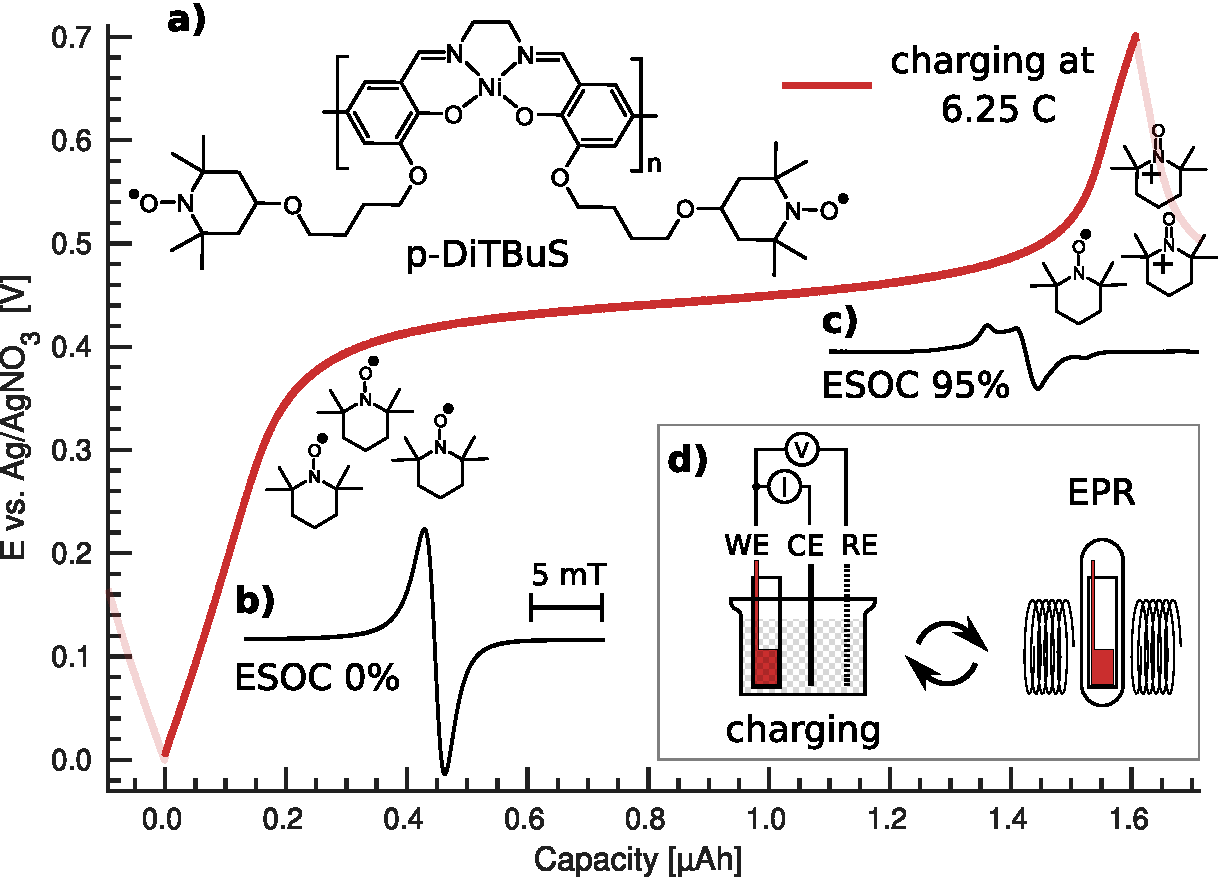
\includegraphics[width=0.7\textwidth]{./introduction/figures/Figure_1.pdf}
	\caption{Galvanostatic charge-discharge curve for a pDiTBuS cathode film at 10~$\muup$A (6.25~C), chemical structure of pDiTBuS (a), normalized cwEPR spectral signatures for reduced (b) and oxidized (c) states. Scheme of the ex-situ EPR measurement on the pDiTBuS half cell (d).}
	\label{fig:Figure_1}
\end{figure}







